\documentclass{standalone}
\usepackage{tikz-timing}
% \usetikztiminglibrary[rising arrows]{clockarrows}
\usetikzlibrary{arrows,calc,decorations.markings}

\pagestyle{empty}

\begin{document}

\pgfarrowsdeclarecombine{|<}{>|}{|}{|}{latex}{latex}
\def\Dimline[#1][#2][#3][#4]{
    \begin{scope}[>=latex] % redef arrow for dimension lines
        \draw let \p1=#1, \p2=#2, \n0={veclen(\x2-\x1,\y2-\y1)} in [|<->|,
        decoration={markings, % switch on markings
                mark=at position .5 with {\node[#3] at (0,0) {#4};},
        },
        postaction=decorate] #1 -- #2 ;
    \end{scope}
}

\begin{tikztimingtable}[scale=1.7]
  Clock             & H 10{1C} 1C\\
  input0            & D{...} 10D{INPUT0} D{...}\\
  input1            & D{...} 10D{INPUT1} D{...}\\
  input             & D{...} 2D{INPUT0} 2D{INPUT1} 2D{INPUT2} 2D{INPUT3} 2D{INPUT4}  D{...}\\
  output0           & 5D{...} 7D{INPUT0}\\
  output1           & 7D{...} 5D{INPUT1}\\
  \extracode
  \tablerules
\end{tikztimingtable}

% \begin{figure}
%     \centering
%     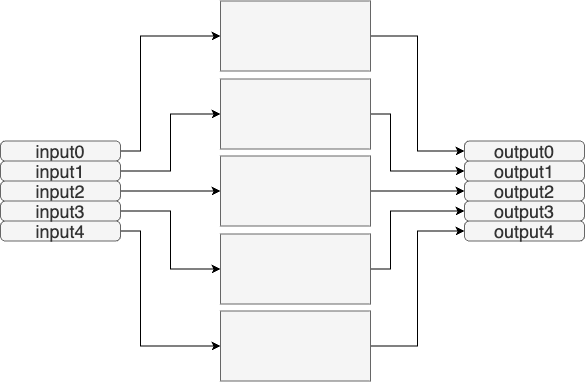
\includegraphics[width=1\textwidth]{../images/sdm.png}
%     \label{fig:original-vhdl-design}
% \end{figure}

\end{document}